
\documentclass[a4paper,12pt]{article}
\frenchspacing
\usepackage{microtype}
\usepackage{graphicx}
\usepackage{placeins}
\graphicspath{ {./images/} }
\usepackage[pdfauthor={Jenny Vermeltfoort},pdftitle={Model based consistency of variable names for improved high-level understanding.}]{hyperref}

\begin{document}

\title{Model based consistency of variable names for improved high-level understanding.}
\author{Jenny Vermeltfoort}
\date{\today}
\maketitle

\section{Introduction}
While software is written to be interpreted by computers it is of key importance that humans are able to quickly understand it fully. The naming of identifiers is an important tools for software engineers to meaningfully transfer concepts to their colleagues, who might be maintaining, updating or refracturing the code. Comprehensibility of these concepts might be restricted by the innate free characteristics of naming conventions within software languages. It is therefore of interest to identify what kind of identifiers are difficult to interpret and whether formal rules may be developed to create a more structured way of transferring concepts.
This report evaluates two research papers that address these issues. The first, written by Floarian Deissenboeck and Markus Pizka, tries to define a formal model to create conise and consistent naming schemas in their paper \textit{Concise and consistent naming}. The second, \textit{Improving Semantic Consistency of Variable Names} with Use-Flow Graph Analysis written by Yusuke Shinyama, Yoshitaka Arahori, and Katsuhiko Gondow builds a probabilistic model to test if a variable name reflects its intended usage pattern. This report summarizes, and produces a compounded conclusion of both papers. At the end of the report a short paragraph describes the approach used for writing this report.

\newpage

\section{Imrpoving Semantic Consistency}
Yusuke Shinyama et al. find that the semantic consistency of variable names in a code base is an important factor for a high level understanding of its concepts. They define an automated method to identify and correct inconsistency’s over a project which has foundations within a multitude of research papers. In short these papers conclude that long descriptive names improve understanding and that inconsistent naming results in a decay of code quality.
The paper is not innovative in its research question, there already exist a couple of methods for identifying inconsistency developed by other researchers. One converts source code in word embeddings and relates it to the natural language, another uses manually crafted rules to detect naming bugs, and another validates whether method names properly describe the method’s code contents. Shinyama et al use a novel approach by trying to identify semantic inconsistency of variable names instead of method names. Accordingly, variable names better infer the project’s meaning and highlevel design.
The paper defines the consistency of a variable by looking at its complete context. The context of a variable is contained within the surrounding code, i.e. the code performs an operation on the variable. This operation is the relation of the variable towards its implementation and its usage. Defining this relation for each variable that exists within a project it becomes possible to compare these relations and make a consistency prediction.
For illustration purposes see the example of a variable name and its context below. The variable name “year\_birth” may be substituted by an arbitrary name “x”. The initial assignment using the method call get\_time\_person and the designation method call calc\_age both form the context. The last two lines of the example thus define the relation of the variable “x” to the context “code”. By comparing all the variables that fit this exact relation, consistency may be determined for any variable within the project.

\begin{verbatim}
    int year_birth = get_time_person(person).year;
    int age = calc_age(year_now, year_birth);

    int x = get_time_person(person).year;
    int age = calc_age(year_now, x);
\end{verbatim}

To support automation of this process the paper proposes a graph structure -- a “Use-Flow Graph” (UFG) -- to describe the context of a variable. See the figure below. The graph depicts the origin, the operations and the designation of the variable. By traversing the lanes from top to bottom for each variable an usage pattern is constructed. This usage pattern is the relation of the variable name towards its context, which as described in the paragraphs before may be used for consistency testing. Certain software specific operations, in this example the mathematical operators, are depicted using unique blocks; think while- and for-loops, if-statements, and method calls. 

\begin{figure}[ht]
    \centering
    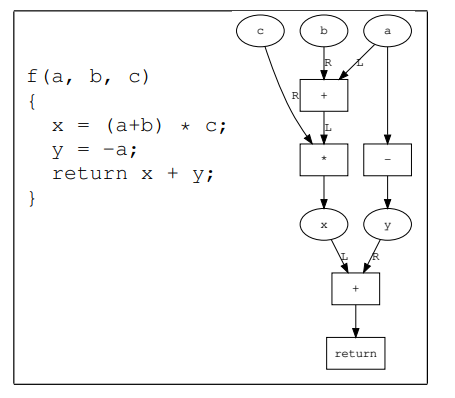
\includegraphics[width=0.7\linewidth]{ufg}
    \caption{example UFG.}
    \label{fig:ufg}
\end{figure}
\hfill
\FloatBarrier

    
The paper shows that the automated method defined by Shinyama et al. is more capable of providing consistent naming with-in a project over human developers. However the authors do note a clause concerning the results; the small pool of nine reviewers might be biased which could have skewed the results; also the method is only designed for Java code and software languages with dynamic dispatch and variable aliasing exceed the model's limitations.

\section{Conclusion}
The article written by Yusuke seems to imply that the meaning of a variable names depends on its usage pattern within the boundaries of its scope – the code base. However, the article of Deissenboeck defines that a variable should be meaningful independent of its context. This juxtaposition depicts the weakness of objectifying a subjective subject. While I agree that some formal rules may improve comprehension of software overall, it seems almost impossible to define some objective schema. Both articles seem to tip their toes into the psychology of naming comprehension, yet both articles lack strong argumentation that is founded upon quantitative data found in psychological research.

\section{Assignment approach}
Here you describe the approach you took in completing this writing assignment. Refer to the steps as discussed in the lecture, and describe how you completed them. Revise this section for assignment 4, adding the steps you took to complete part 2 of the writing assignment. 

% the bibliography
\bibliographystyle{plain}
\bibliography{references}

\end{document}

